\begin{center}
\textit{by Jeong Han Kim, Minho Kim, Kyoungchul Kong, Konstantin
  T. Matchev, Myeonghun Park}
\end{center}


In this section, we discuss the discovery prospects for double Higgs production in the $hh \to (b\bar b) (W W^*)$ channel. In order to increase sensitivity in the dilepton channel \cite{CMS:2015nat,CMS:2017cwx,Adhikary:2017jtu}, we propose a novel kinematic method, which relies on two new kinematic functions, {\it Topness} and {\it Higgsness} \cite{Kim:2018cxf}. They characterize features of the major ($t\bar t$) background and of $hh$ events, respectively. The method also utilizes two less commonly used variables, the subsystem $M_{T2}$ (or subsystem $M_2$) \cite{Lester:1999tx,Burns:2008va,Barr:2011xt} for $t\bar t$ and the subsystem $\sqrt{\hat {s}}_{min}$ (or subsystem $M_1$) \cite{Konar:2008ei,Konar:2010ma,Barr:2011xt} for $hh$ production.
%
For any given event, Topness \cite{Graesser:2012qy,Kim:2018cxf} quantifies the degree of consistency to dilepton $t\bar t$ production, where there are 6 unknowns (the three-momenta of the two neutrinos, $\vec p_{\nu}$ and $\vec p_{\bar\nu}$) and four on-shell constraints, for
$m_t$, $m_{\bar t}$, $m_{W^+}$ and $m_{W^-}$, respectively. The neutrino momenta can be fixed by minimizing the quantity 
%
\begin{eqnarray}
\chi^2_{ij} \equiv \min_{\tiny \mptvec = \vec p_{\nu T} + \vec p_{ \bar\nu T}}  \left [ 
\frac{\left ( m^2_{b_i \ell^+ \nu} - m^2_t \right )^2}{\sigma_t^4}    +
\frac{\left ( m^2_{\ell^+ \nu} - m^2_W \right )^2}{\sigma_W^4}   \label{eq:tt}  
 + \frac{\left ( m^2_{b_j \ell^- \bar \nu} - m^2_t \right )^2}{\sigma_t^4}  +
\frac{\left ( m^2_{\ell^- \bar\nu} - m^2_W \right )^2}{\sigma_W^4}   \right ]  , 
\end{eqnarray}
%
subject to the missing transverse momentum constraint, $ \mptvec = \vec p_{\nu T} + \vec p_{ \bar\nu T}$. 
Since there is a twofold ambiguity in the paring of a $b$-quark and a lepton, we define {\it Topness} as the smaller of the two $\chi^2$s,
\begin{eqnarray}
T &\equiv&  { \min} \left ( \chi^2_{12} \, , \, \chi^2_{21} \right ) \, .
\end{eqnarray}

In double Higgs production, the two $b$-quarks arise from a Higgs decay ($h \to b \bar b$), and therefore their invariant mass $m_{bb}$
can be used as a first cut to enhance the signal sensitivity. 
For the decay of the other Higgs boson, $h \to W W^* \to \ell^+ \ell^- \nu \bar\nu$, we define {\it Higgsness} \cite{Kim:2018cxf} as follows: 
%
\begin{eqnarray}
H &\equiv&    {\rm min} \left [
 \frac{\left ( m^2_{\ell^+\ell^-\nu \bar\nu} - m^2_h \right )^2}{\sigma_{h_\ell}^4}    \right. 
 + \frac{ \left ( m_{\nu  \bar\nu}^2 -  m_{\nu\bar\nu, peak}^2 \right )^2}{ \sigma^4_{\nu}}
 \label{eq:hww}   \\
 && \hspace*{-1cm}  \left. + {\min} \left ( 
\frac{\left ( m^2_{\ell^+ \nu } - m^2_W \right )^2}{\sigma_W^4} + 
\frac{\left ( m^2_{\ell^- \bar \nu} - m^2_{W^*, peak} \right )^2}{\sigma_{W^*}^4}  \, , 
\frac{\left ( m^2_{\ell^- \bar \nu} - m^2_W \right )^2}{\sigma_W^4} + 
\frac{\left ( m^2_{\ell^+ \nu} - m^2_{W^*, peak} \right )^2}{\sigma_{W^*}^4}  
\right )  \right ]   \, , \nonumber
\end{eqnarray}
%
%
where $m_{W^*}$ is the invariant mass of the lepton-neutrino pair which resulted from the off-shell $W$. 
It satisfies $0 \leq m_{W^*} \leq m_h- m_W$ and $m_{W^*}^{peak} = \frac{1}{\sqrt{3}} \sqrt{ 2 \left ( m_h^2 + m_W^2 \right ) - \sqrt{m_h^4 + 14 m_h^2 m_W^2 + m_W^4}}$ is the peak in the $m_{W^*}$ distribution.
$m_{\nu\bar\nu}^{peak} = m_{\ell\ell}^{peak} \approx 30$ GeV is the location of the peak in the $\frac{\textrm{d}\sigma}{\textrm{d} m_{\nu\bar\nu}}$ or $\frac{\textrm{d}\sigma}{\textrm{d} m_{\ell\ell}}$ distribution \cite{Kim:2018cxf,Cho:2012er}.
%, which is bounded from above by $m_{\nu\bar\nu}^{max} = m_{\ell\ell}^{max} = \sqrt{m_h^2 - m_W^2}$.
%
%The phase space distribution of $\frac{\textrm{d}\sigma}{\textrm{d}m_{\nu \bar\nu}}$ is given by $\frac{\textrm{d}\sigma}{\textrm{d}m_{\nu \bar\nu}} \propto \int\textrm{d}m_{W^*}^2 \lambda^{1/2}(m_h^2,m_W^2, m_{W^*}^2) f(m_{\nu \bar\nu})$, where $\lambda(x,y,z)=x^2+y^2+z^2-2xy-2yz-2zx$ is the two-body phase space function and $f(m)$ is the invariant mass distribution of the antler topology with $h\to W W^* \to \ell^+ \ell^- \nu \bar \nu$
%
%\begin{eqnarray}
%f(m)\sim \left\{
%\begin{array}{l l}
%\eta\, m \, , & 0 \leq m \leq e^{-\eta}E, \\ [1mm]
%m \ln(E/m)  \, , & e^{-\eta}E \leq m \leq E,
%\end{array}\right.  \label{eq:antlerf}
%\end{eqnarray}
%
%where the endpoint $E$ and the parameter $\eta$ are defined in terms of the particle masses as $E =  \sqrt{ m_W m_{W^*} \, e^{\eta}} $ and $\cosh \eta =\left ( \frac{m_h^2- m_{W}^2 - m_{W^*}^2}{2 m_{W} m_{W^*} } \right )$ \cite{Cho:2012er}. 
%
%
%The actual peak of 30 GeV is slightly less than the result for pure phase space due to a helicity suppression in the $W$-$\ell$-$\nu$ vertex. 
%

The $\sigma$ values in Eqs.\,(\ref{eq:tt}) and (\ref{eq:hww}) result from the experimental uncertainties and intrinsic particle widths. In principle, they can be treated as free parameters and tuned using a neutral network (NN), a boosted decision tree (BDT), etc. In our numerical study, we use $\sigma_t=5$ GeV, $\sigma_W=5$ GeV, $\sigma_{W^*}=5$ GeV, $\sigma_{h_\ell}=2$ GeV, and $\sigma_\nu = 10 $ GeV. 
The main contribution in Eq.\,(\ref{eq:hww}) comes from the on-shell conditions for the Higgs and the $W$, while the effects of the invariant mass of the two neutrinos and the off-shell $W$ are minor. 

Along with Higgsness and Topness, we adopt the subsystem $\hat{s}_{min}^{(\ell\ell)}$ for $h \to W^\pm W^{*\mp}\to\ell^+\ell^- \nu \bar \nu$ \cite{Konar:2008ei,Konar:2010ma} and the subsystem $M_{T2}$ for the $b \bar b$ system ($M_{T2}^{(b)}$) and the lepton system ($M_{T2}^{(\ell)}$) \cite{Burns:2008va}. 
%
The variable $ \hat{s}_{min}^{({\rm v})} $ is defined as $ \hat{s}_{min}^{({\rm v})} = m_{{\rm v}}^2 + 2 \left ( \sqrt{ |\vec P_{T}^{\rm v} |^2 + m_{\rm v}^2 }  |\mptvec| - \vec P_{T}^{\rm v} \cdot \mptvec \right )$ \cite{Konar:2008ei,Konar:2010ma,Barr:2011xt}, where $({\rm v})$ represents a set of visible particles under consideration, while $m_{\rm v}$ and $\vec P_{T}^{\rm v}$ are their invariant mass and transverse momentum, respectively. It provides the minimum value of the Mandelstam invariant mass $\hat s$ which is consistent with the observed visible 4-momentum vector.
%
The $M_{T2}$ is defined as 
$M_{T2} (\tilde m) \equiv \min\left\{\max\left[M_{TP_1}(\vec{p}_{\nu T},\tilde m),\;M_{TP_2} (\vec{p}_{\bar\nu T},\tilde m)\right] \right\}$ where $\tilde m$  is the test mass for the daughter particle and the minimization over the transverse masses of the parent particles $M_{TP_i}$ ($i=1, 2$) is performed over the transverse neutrino momenta $\vec{p}_{\nu T}$ and $\vec{p}_{\bar\nu T}$ subject to the 
$\mptvec $ constraint  \cite{Lester:1999tx,Burns:2008va,Barr:2011xt,Debnath:2017ktz,Konar:2009wn,Konar:2009qr,Cho:2007qv}. 


%
\begin{figure*}[t]
\centering
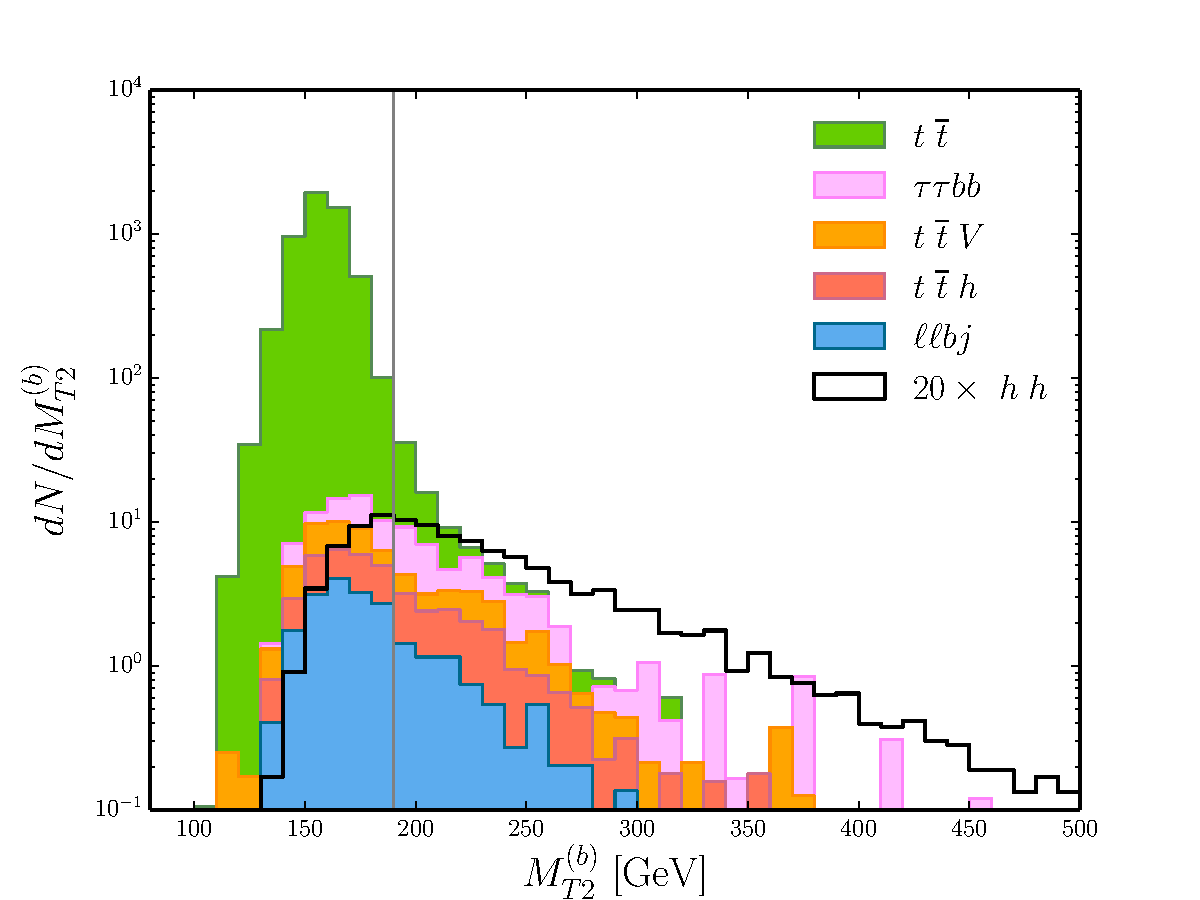
\includegraphics[width=5.77cm]{\main/section3/plots/Stacked_Log_MT2_b_Zero_BaseLineSel.pdf} \hspace*{-0.65cm}
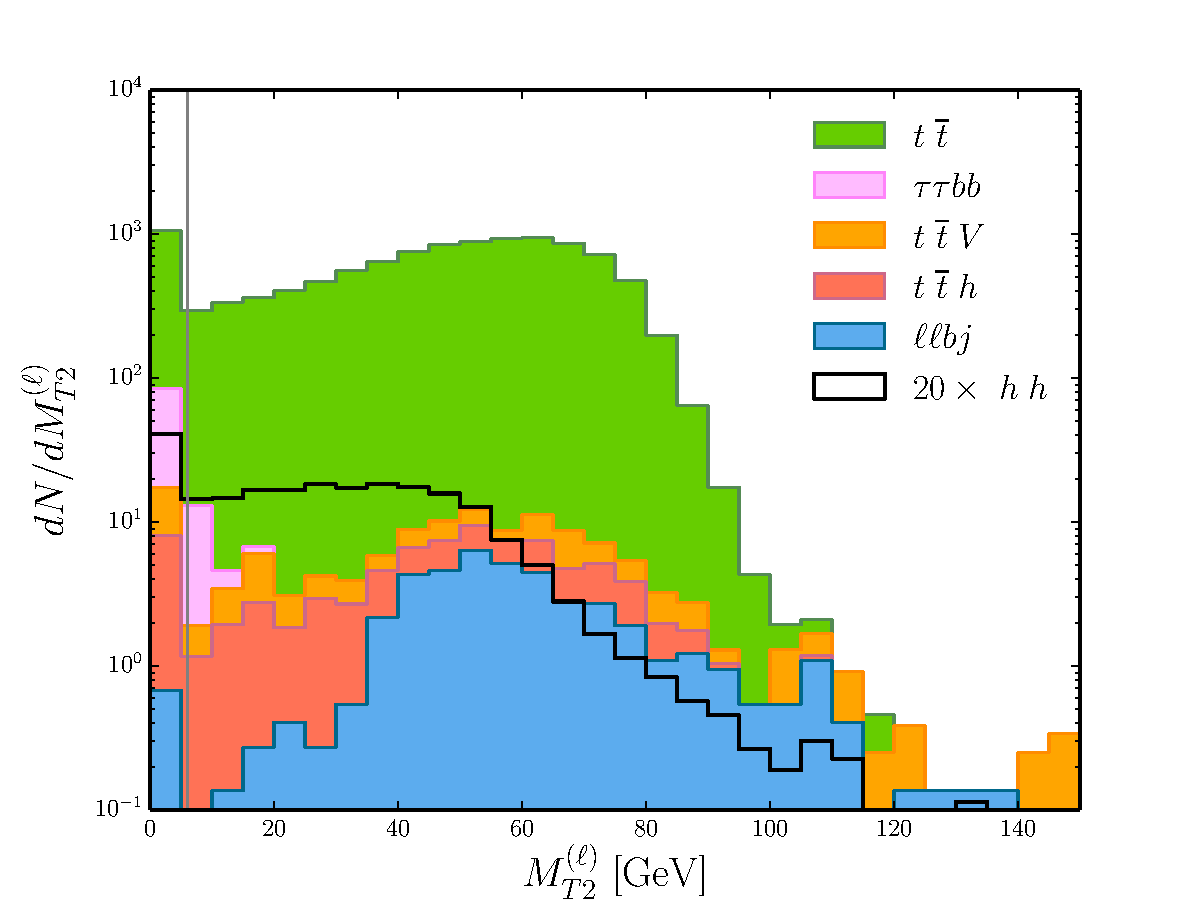
\includegraphics[width=5.77cm]{\main/section3/plots/Stacked_Log_MT2_l_Zero_BaseLineSel.pdf}   \hspace*{-0.65cm}
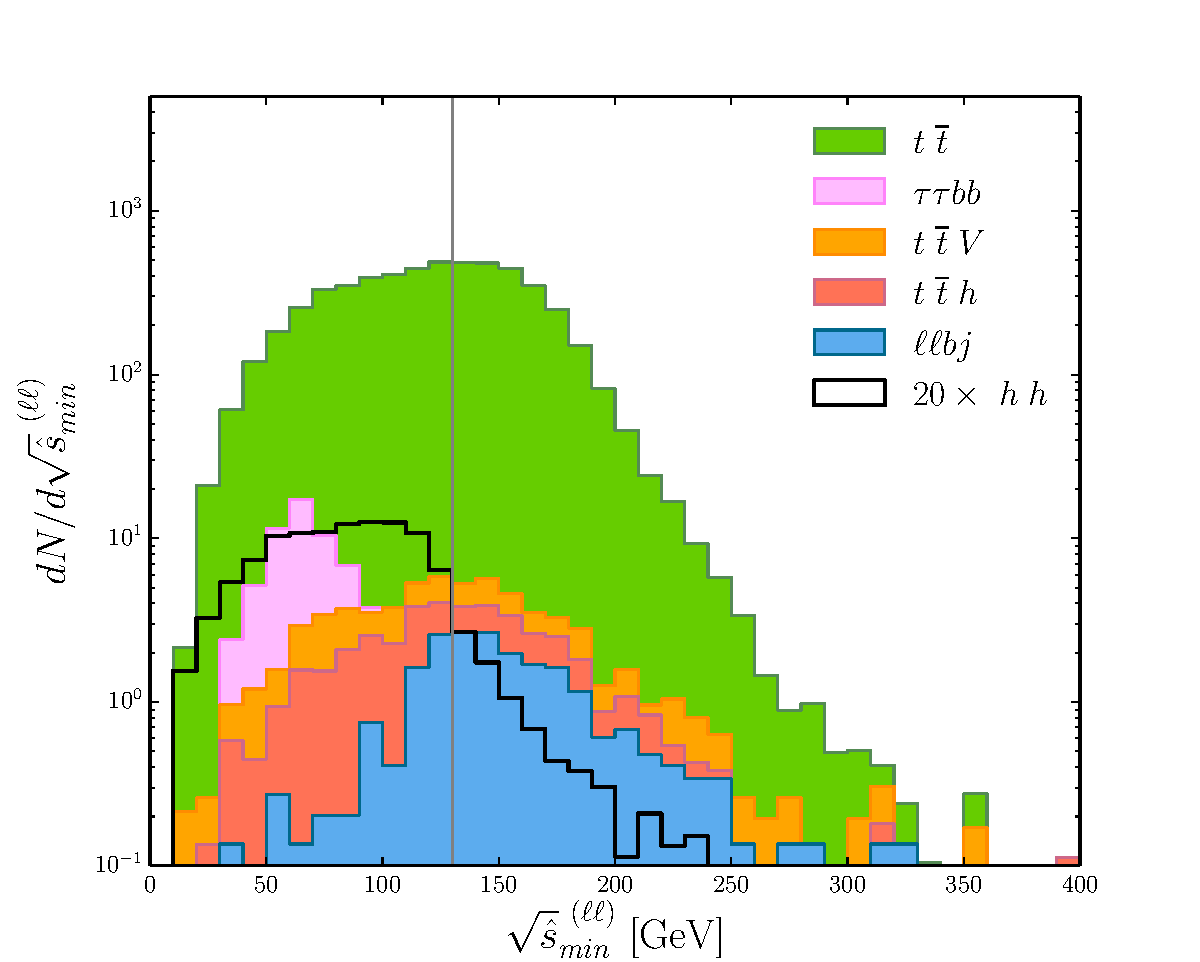
\includegraphics[width=5.4cm]{\main/section3/plots/Stacked_Log_Smin_ll_Zero_BaseLineSel.pdf} 
\caption{\label{fig:newcuts} 
Distributions for signal ($hh$) and all backgrounds ($t \bar t$, $t\bar t h$, $t \bar t V$, $\ell\ell b j$ and $\tau\tau b b$) for $M_{T2}^{(b)}$, $M_{T2}^{(\ell)}$ and $\sqrt{\hat{s}}_{min}^{(\ell\ell)}$ after loose baseline selection cuts defined in Ref. \cite{Kim:2018cxf}. 
The vertical lines at $M_{T2}^{(b)} = 190$ GeV, $M_{T2}^{(\ell)}= 6$ GeV and $\sqrt{\hat{s}}_{min}^{(\ell\ell)}=130$ GeV mark the optimized cuts.}
\end{figure*}
%
%
%
\begin{figure}[t]
\centering
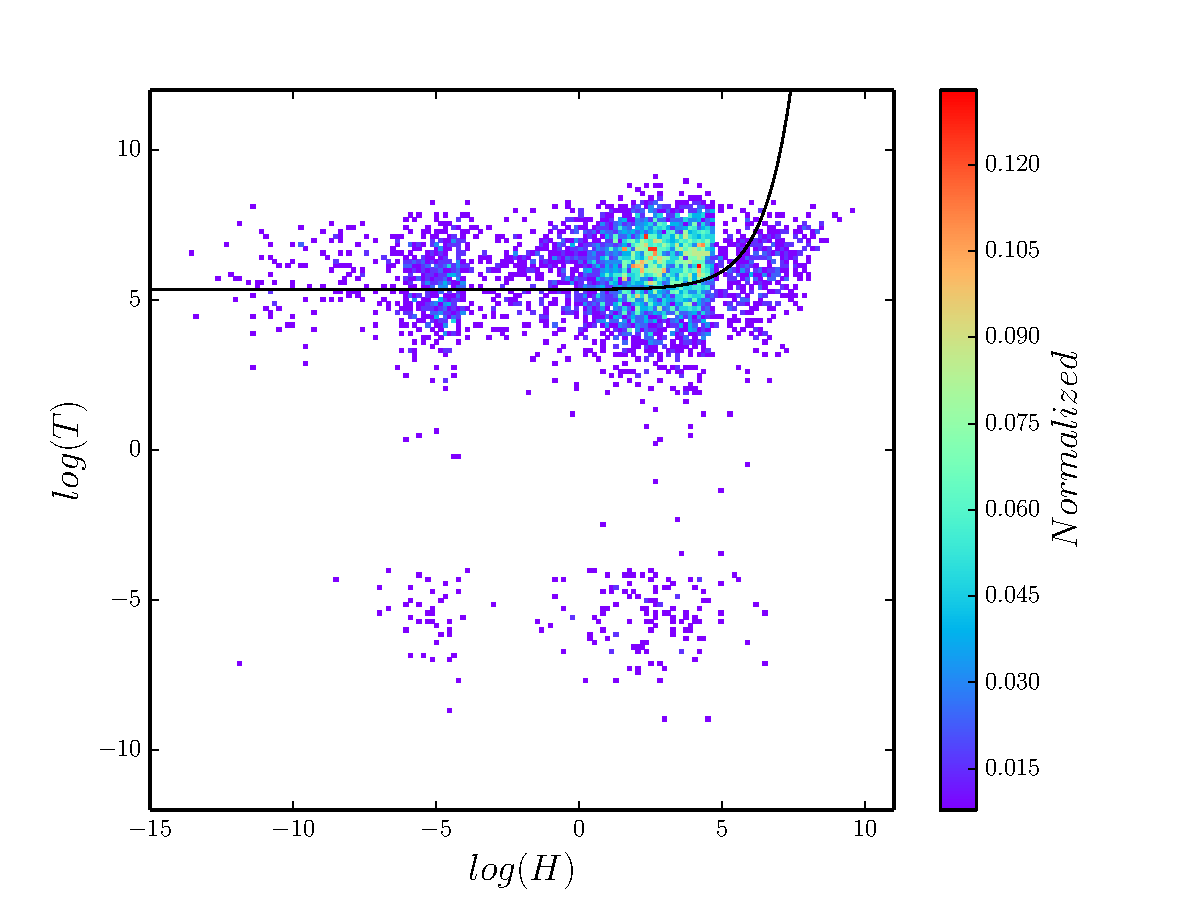
\includegraphics[width=5.4cm]{\main/section3/plots/Scatter_hh_Zero_BaseLineSel.pdf}   \hspace*{-0.525cm}
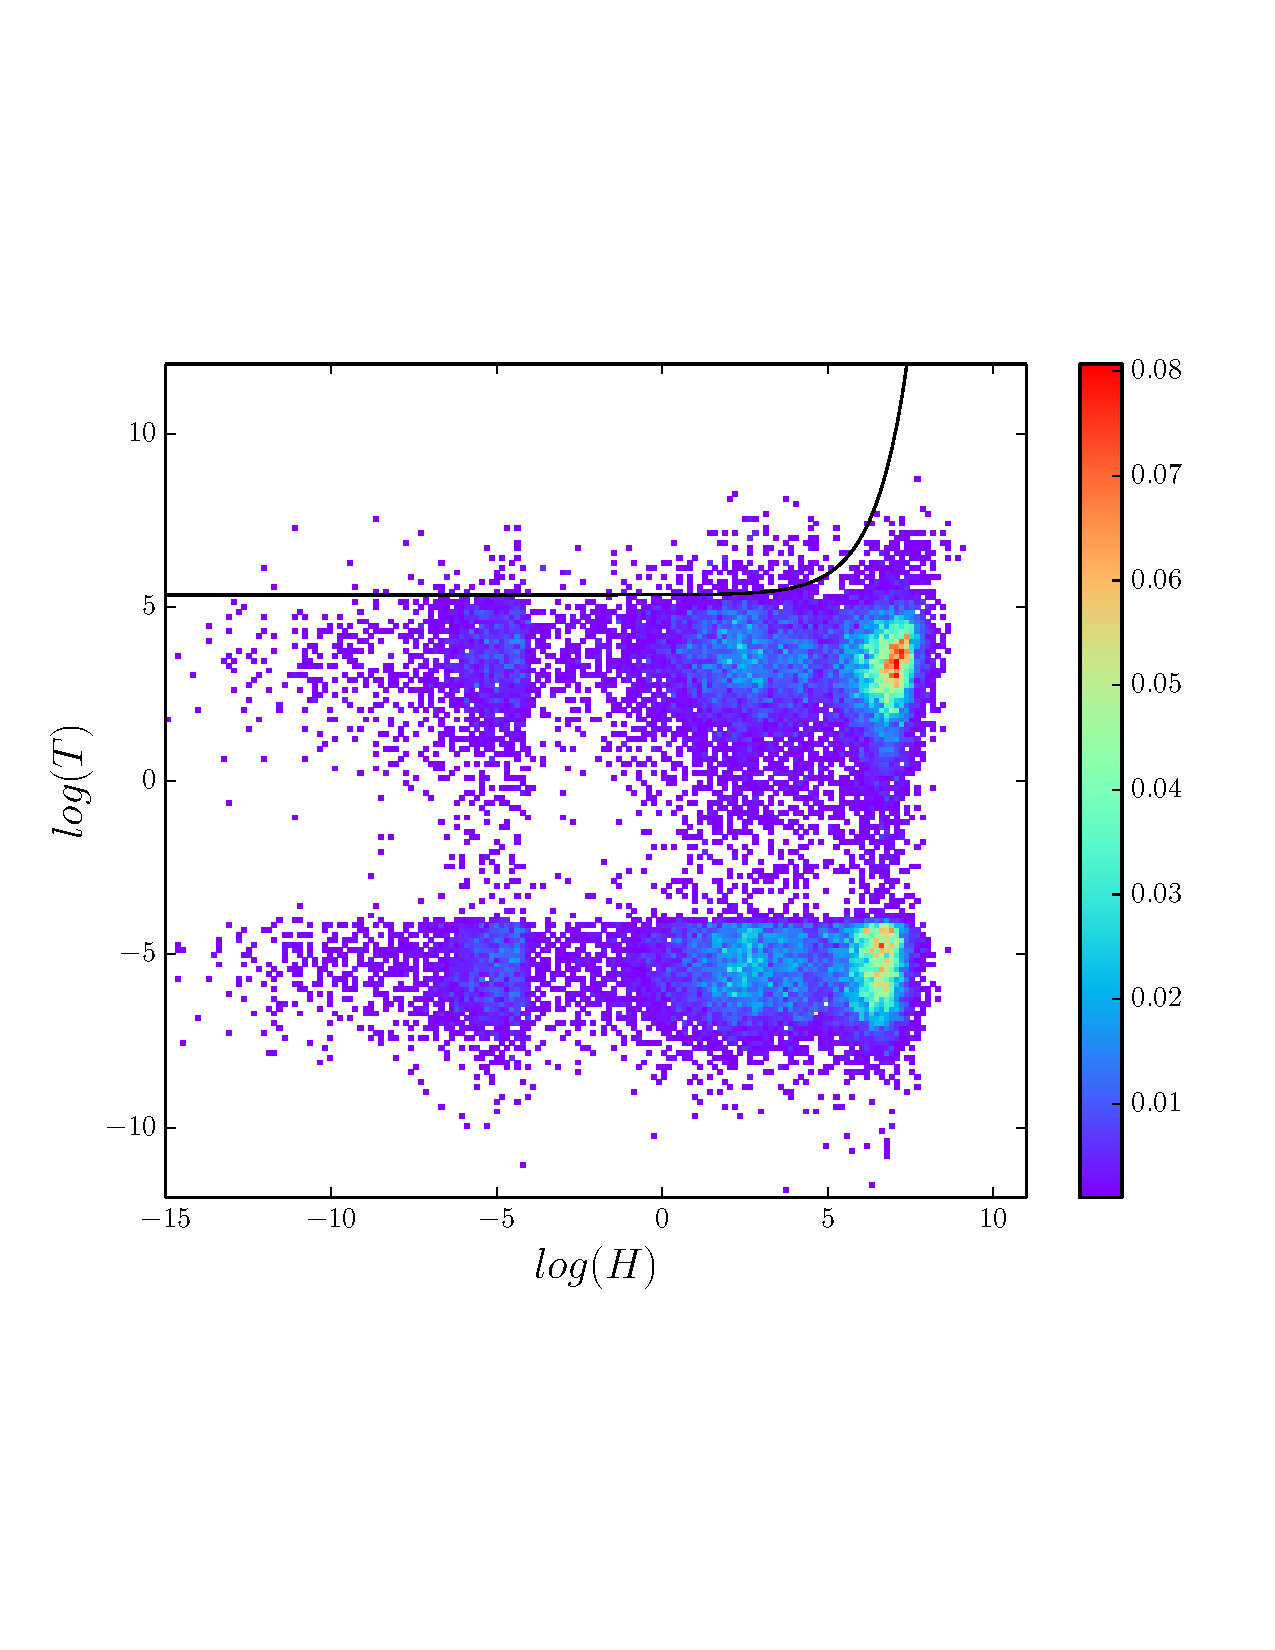
\includegraphics[width=5.2cm]{\main/section3/plots/Scatter_BGD_Zero_BaseLineSel.pdf} \hspace*{-0.1cm}
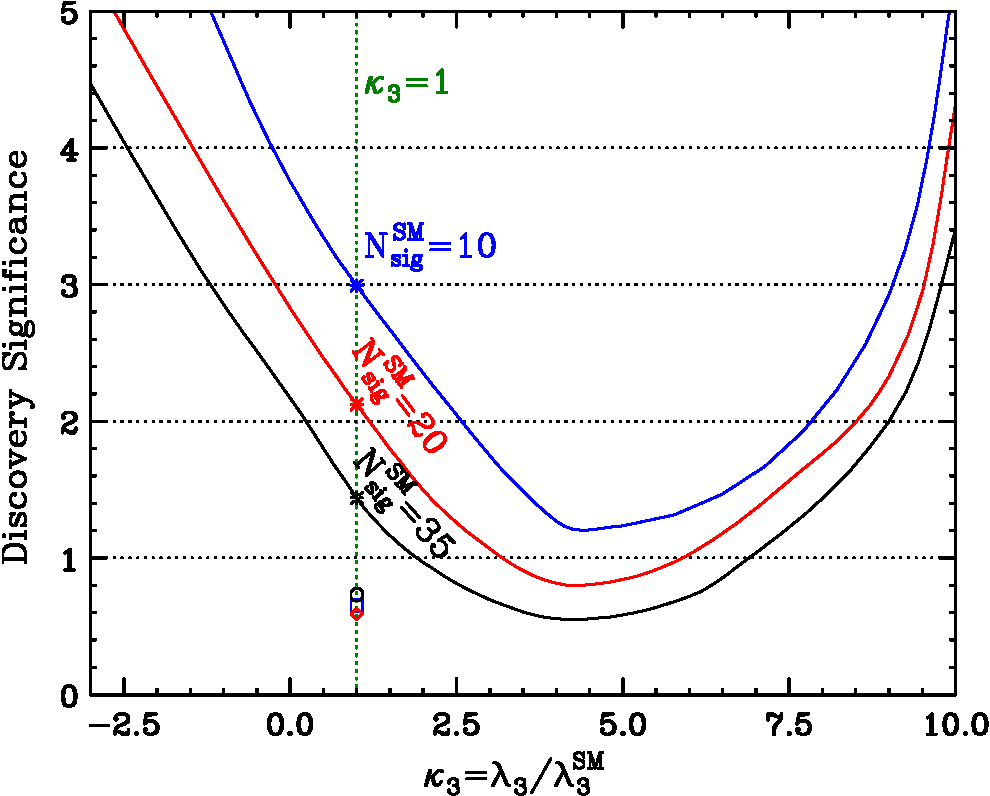
\includegraphics[width=5.25cm]{\main/section3/plots/kappa3_report.pdf} 
\caption{\label{fig:scatter} 
Scatter distribution of ($\log H$, $\log T$) for signal ($hh$ in the left) and backgrounds ($t \bar t$, $t\bar t h$, $t \bar t V$, $\ell\ell b j$ and $\tau\tau b b$ in the middle) after loose baseline selection cuts.
The right panel shows the expected discovery significance at the 14 TeV LHC with 3 ab$^{-1}$ as a function of the triple Higgs coupling $\kappa_3$.
We obtain each curve by applying the same set of cuts optimized for the SM point ($\kappa_3=1$) to non-SM points ($\kappa_3 \neq 1$) for ${\rm N_{sig}^{SM}}=35$ in black, ${\rm N_{sig}^{SM}}=20$ in red and ${\rm N_{sig}^{SM}}=10$ in blue.
%The yellow (cyan) shade represents 95\% CL exclusion of $\kappa_3$ in the $bb\gamma\gamma$ channel \cite{ATL-PHYS-PUB-2017-001} ($bbbb$ channel \cite{ATL-PHYS-PUB-2016-024}) at the HL-LHC. 
The curves in the left and middle panel are the optimized cuts for the ${\rm N_{sig}^{SM}}=20$ case.
The three symbols {\color{red}$\Diamond$}, {\color{black}$\bigcirc$} and {\color{blue}$\square$} display the signal significance 
using CMS-NN \cite{CMS:2015nat}, CMS-BDT \cite{CMS:2017cwx} and BDT \cite{Adhikary:2017jtu}, respectively.
}
\end{figure}
%

Events for the signal and all relevant background processes were simulated as described in Ref.~\cite{Kim:2018cxf}. After basic selection cuts, we use the kinematic information  discussed above for further background suppression. Distributions of $M_{T2}^{(b)}$, $M_{T2}^{(\ell)}$ and $\sqrt{\hat{s}}_{min}^{(\ell\ell)}$ are shown in Fig.~\ref{fig:newcuts}, while scatter distributions of Topness and Higgsness are displayed in Fig.~\ref{fig:scatter}. 
%
The right panel in Fig.~\ref{fig:scatter} shows the expected signal significance at the HL-LHC as a function of the triple Higgs coupling $\kappa_3$. We obtain each curve by applying the same set of cuts optimized for the SM point ($\kappa_3=1$) to non-SM points ($\kappa_3 \neq 1$) for ${\rm N_{sig}^{SM}}=35$ in black, ${\rm N_{sig}^{SM}}=20$ in red and ${\rm N_{sig}^{SM}}=10$ in blue. The three symbols {\color{red}$\Diamond$}, {\color{black}$\bigcirc$} and {\color{blue}$\square$} show the signal significance using CMS-NN \cite{CMS:2015nat}, CMS-BDT \cite{CMS:2017cwx} and BDT \cite{Adhikary:2017jtu}, respectively.




%
\begin{figure}[t]
\centering
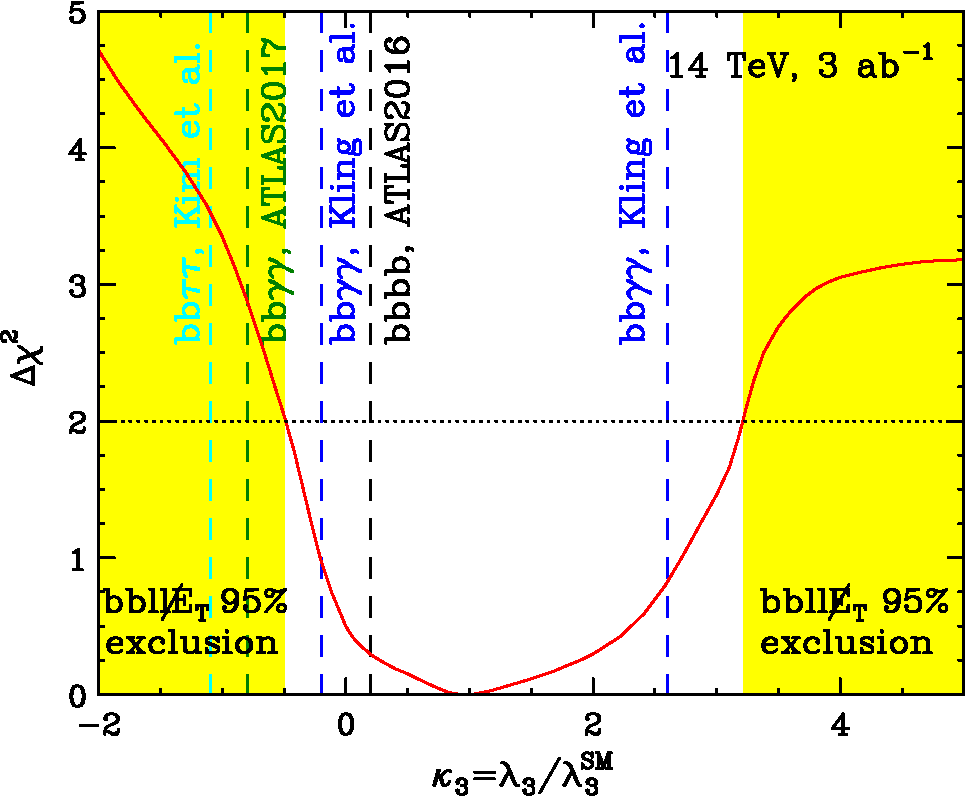
\includegraphics[width=5cm]{\main/section3/plots/precision_14.pdf}   \hspace*{0.cm}
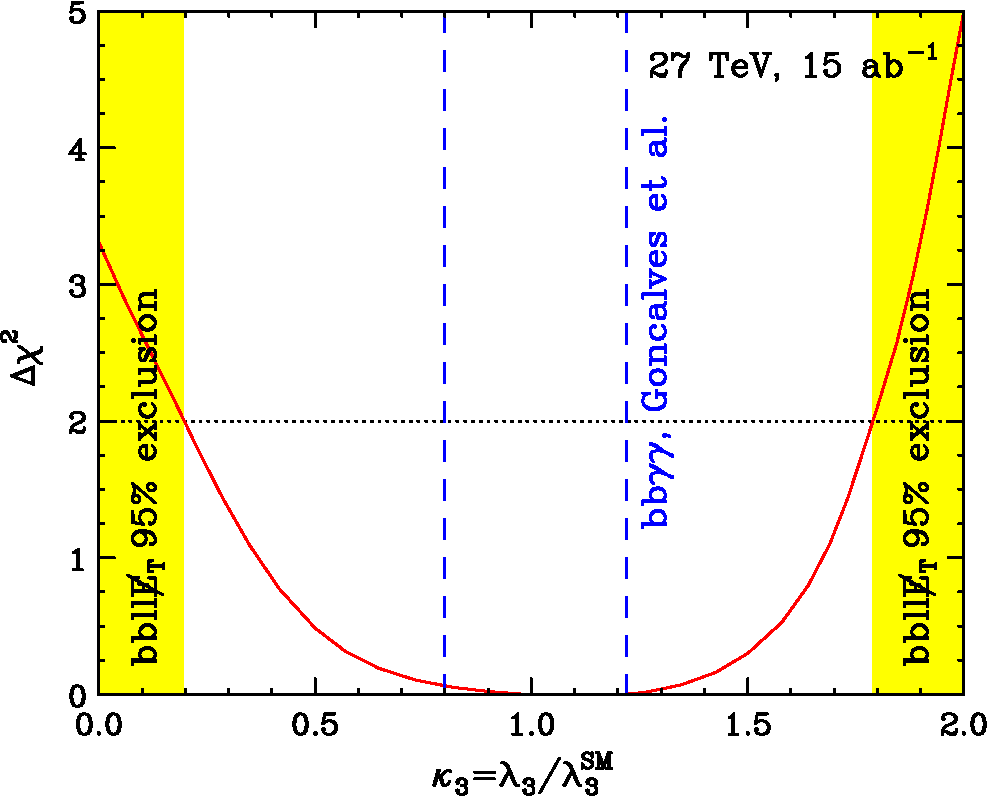
\includegraphics[width=5.03cm]{\main/section3/plots/precision_27.pdf}   \hspace*{-0.cm}
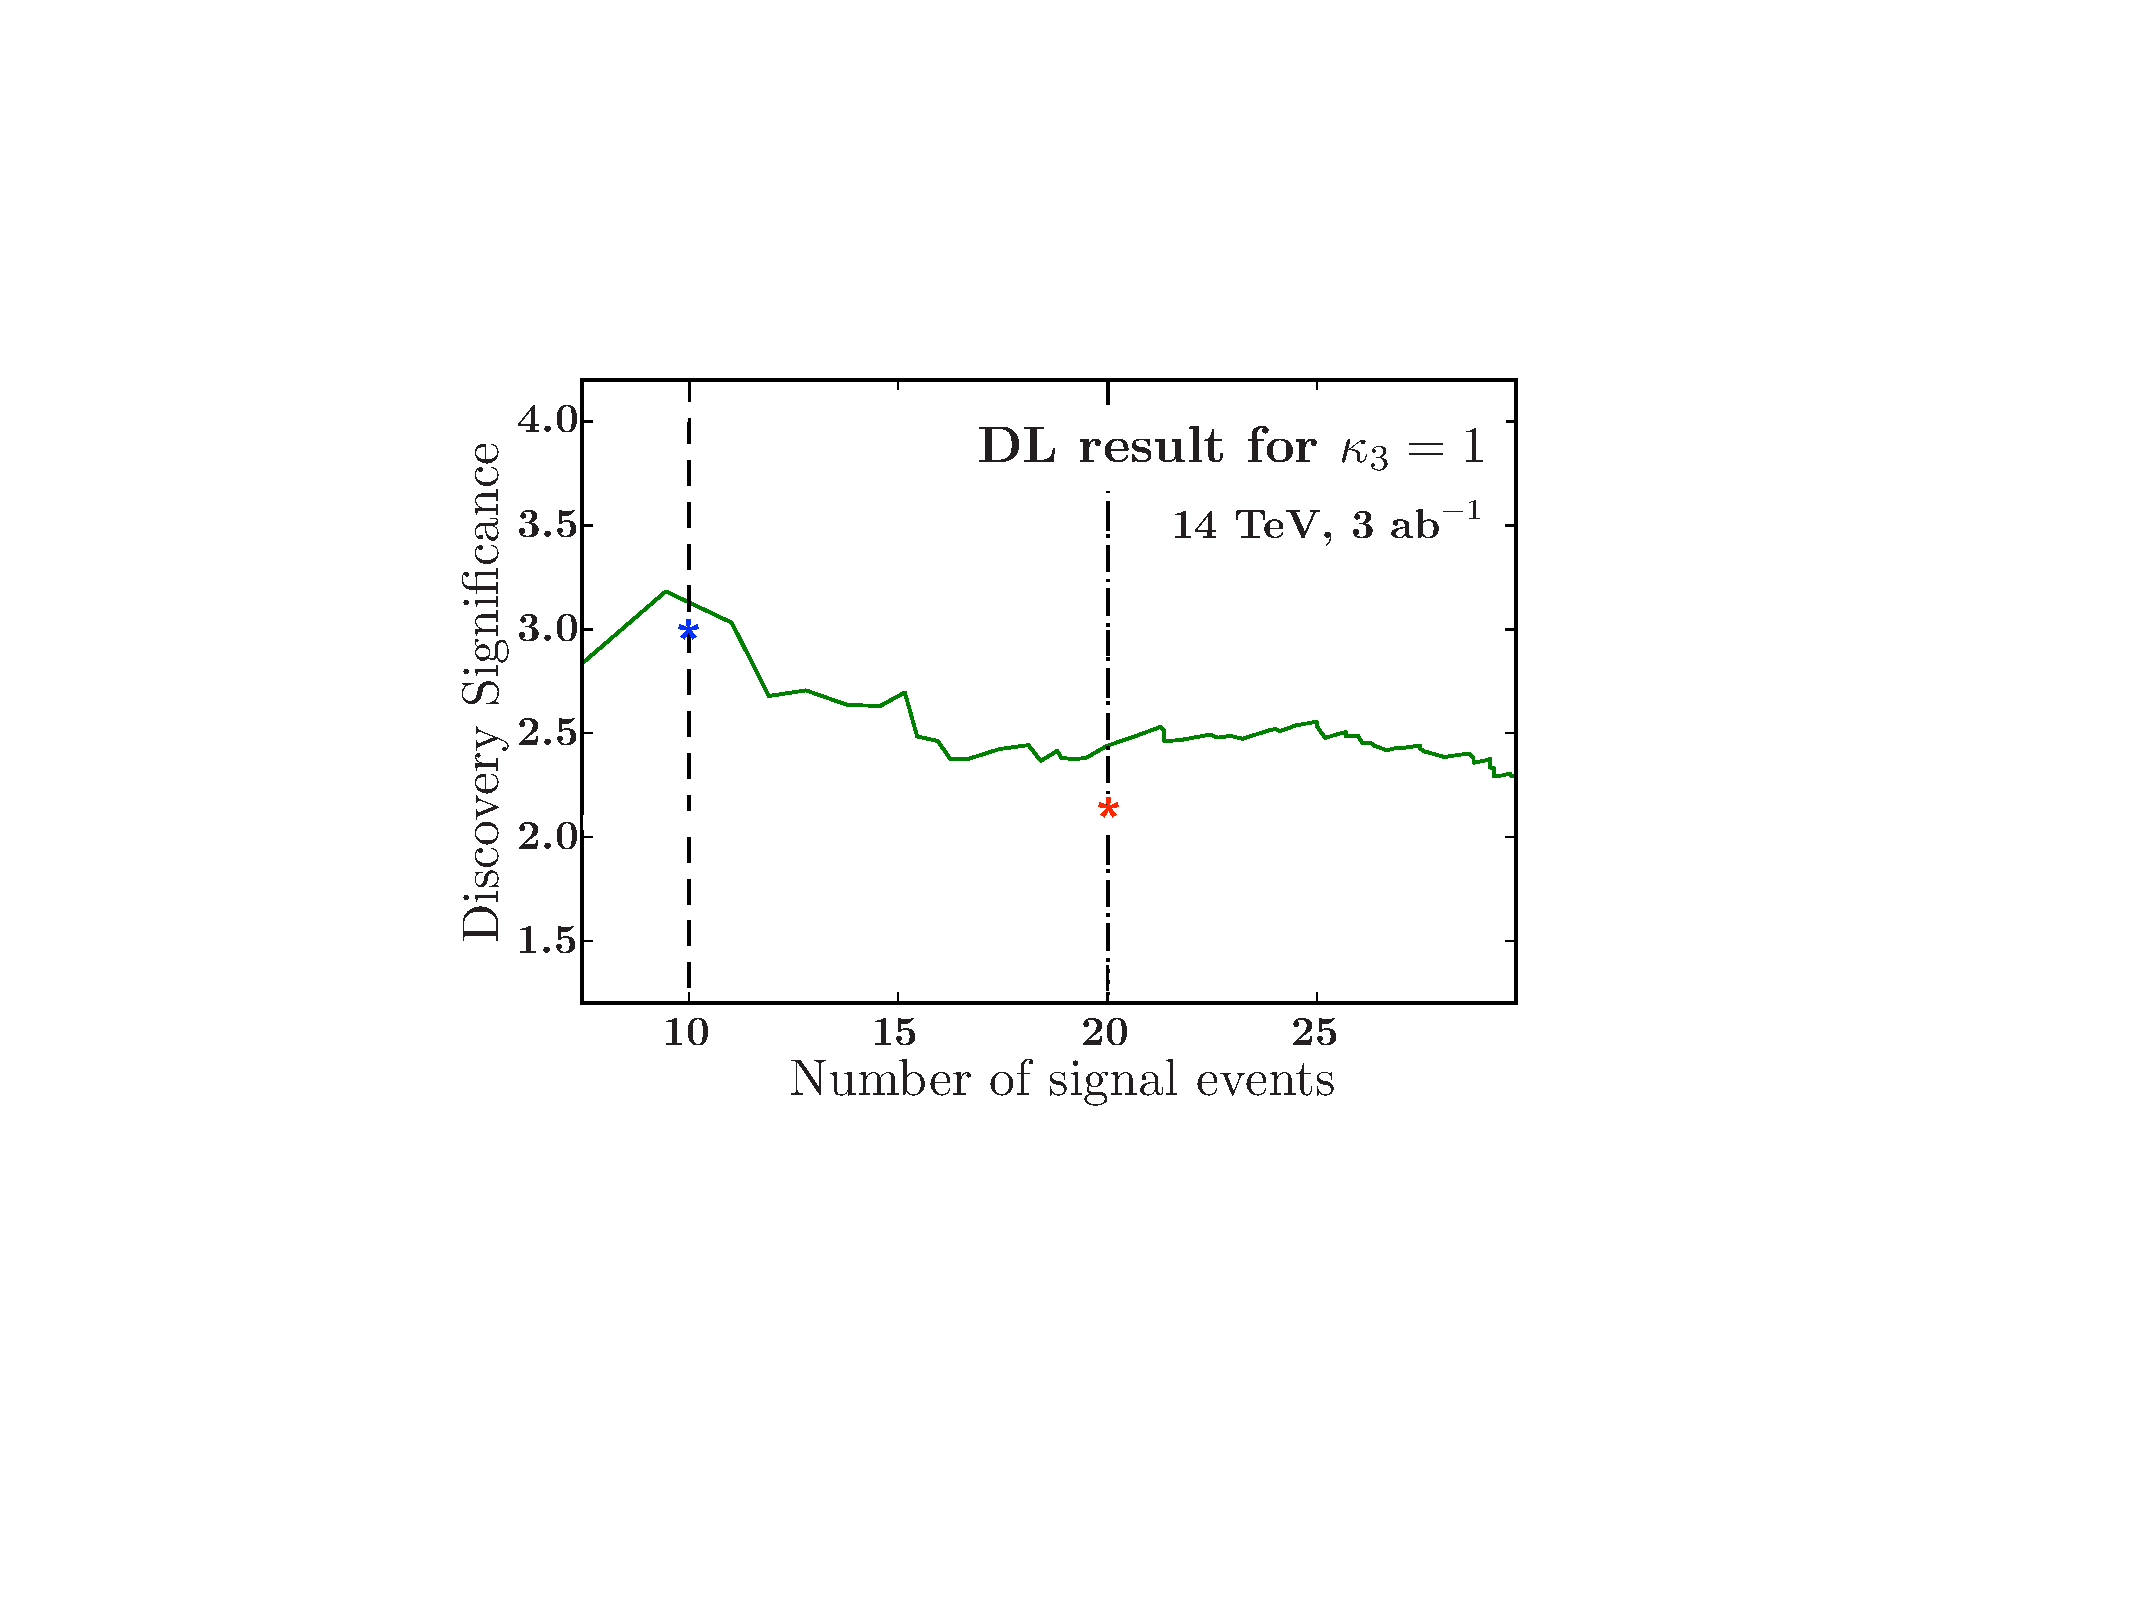
\includegraphics[width=5.2cm,height=4.cm]{\main/section3/plots/dl.pdf}   
\caption{\label{fig:k3precision} 
Significance for observing an anomalous Higgs self-coupling at the 14 TeV LHC with an integrated luminosity of 3 ab$^{-1}$ (left) and at 27 TeV with 15 ab$^{-1}$ (middle).
%The HL-LHC (27 TeV collider) will rule out the Higgs self-coupling outside the range $(-0.5, 3.2)$ ($(0.5, 1.6)$). 
Right: the effect of using a Deep Learning algorithm to improve the discovery significance for $\kappa_3=1$ shown in 
the right panel of Fig.~\ref{fig:scatter}.
}
\end{figure}
%

Finally Fig.~\ref{fig:k3precision} shows the significance for observing an anomalous Higgs self-coupling at the 14 TeV LHC with an integrated luminosity of 3 ab$^{-1}$ and at 27 TeV with 15 ab$^{-1}$, respectively. 
For the HL-LHC, we follow the analysis presented in Ref.~\cite{Kim:2018cxf}.
The red solid curves are obtained with nominal efficiencies for $b$ (mis-)tagging ($\epsilon_{b \to b} = 0.7$, $\epsilon_{c \to b} = 0.2$ and $\epsilon_{j \to b} = 0.01$) \cite{Sirunyan:2017ezt}. 
%, while the (red, dotted) curves are based on the improved efficiencies ($\epsilon_{b \to b} = 0.7$, $\epsilon_{c \to b} = 0.112$ and $\epsilon_{j \to b} = 0.0055$) \cite{Aaboud:2018knk}. 
The HL-LHC will rule out the Higgs self-coupling outside the range $(-0.5, 3.2)$. The four vertical dashed lines in the left panel represent the expected 95\% CL exclusion of $\kappa_3$ in the $bbbb$ channel (black, from Ref. \cite{ATL-PHYS-PUB-2016-024}), in the $bb\gamma\gamma$ channel (blue, from Ref. \cite{Kling:2016lay} and green from Ref.~\cite{ATL-PHYS-PUB-2017-001}) and in the $bb\tau\tau$ channel (cyan, from Ref. \cite{Kim:2018uty}). We notice that the sensitivity in the $bbWW^*$ channel is comparable to the sensitivity in those other channels.  
For the 27 TeV study, we normalize our signal cross section to $139.9$ fb \cite{Grazzini:2018bsd}, and use $K$ factors of $K=1.56$ for $t\bar t$ production \cite{27TeV:ttbar}, $K=1.28$ for $t\bar  t h$ \cite{Demartin:2014fia}, $K=1.54$ for $t \bar t V$ and a conservative $K=2$ for $\ell\ell b \bar b$ and $\tau\tau b\bar b$ \cite{Kim:2018cxf}. 
Our result shows that the 27 TeV collider could observe double Higgs production at 5$\sigma$ for a wide range of values for $\kappa_3$ and would be able to exclude $\kappa_3$ outside the range $(0.2, 1.8)$ (for a comparative study in the $bb\gamma\gamma$ channel, see Ref.~\cite{Goncalves:2018qas} (vertical, dashed lines in the middle panel)).


In summary, we obtained a significant increase in the signal sensitivity for $hh$ production in the dilepton channel compared to previous analyses \cite{CMS:2015nat,CMS:2017cwx,Adhikary:2017jtu}. 
%We checked our results obtained by cut-and-count are in agreement with those obtained by using BDT along with Topness, Higgsness, $M_{T2}^{(b)}$, $M_{T2}^{(\ell)}$ and $\sqrt{\hat{s}}_{min}^{(\ell\ell)}$. 
The method can be easily incorporated into more advanced algorithms for further improvement. 
For example, using deep learning (convolutionary neutral network) slightly improves the discovery significance, see the right panel of Fig.~\ref{fig:k3precision}.
The discussed method is very general and can be easily applied to other processes such as the semi-leptonic final state, resonant $hh$ production, non-resonant production with more than one Higgs boson, etc. It is straightforward to generalize the idea to different topologies in searches for other BSM particles as well.









